\chapter{Introduction}

\section{Motivation and Objectives}

A long term goal of artificial intelligence (AI) is the development of artificial general intelligence (AGI). Since the field's inception in the 1950s, it has swung between hype and breakthroughs, followed by disappointment and reduced funding, known as AI winters \cite{Knight2016}. During the first period of hype from the 50s to the early 70s, Marvin Minsky made the following prediction: \cite{Darrach}

\begin{quote} 
\centering 
``In from three to eight years we will have a machine with the general intelligence of an average human being." - Marvin Minsky, 1970
\end{quote}

This prediction was clearly not realised, and the first AI winter would shortly follow.

Symbolic AI was developed during this winter, which encodes knowledge as human-readable rules and facts, making it easy to comprehend chains of actions and abstract relationships \cite{Reingold2001}. For instance, given the unary relations \texttt{red} and \texttt{strawberry}, and the binary relation \texttt{bigger}, we can say that \texttt{A} is the smallest red strawberry by writing $$\texttt{red(A)} \quad \texttt{strawberry(A)} \quad \forall\texttt{B bigger(B, A)}$$ But given the unary relations \texttt{yellow} and \texttt{banana} we could also write that \texttt{A} is the third biggest yellow strawberry, or a red banana, and so on. We can see that the rules and facts in symbolic logic can be endlessly recombined and extended. This allows for the manipulation of high-level abstract concepts, which is key to AGI \cite{Garnelo2016}.

However, symbolic AI has a major philosophical problem: the facts and rules are only meaningful to the human writing them; their meaning is not intrinsic to the system itself. This is known as the \textit{symbol grounding problem}.

Today we find ourselves in yet another period of hype and exciting breakthroughs not afflicted by the symbol grounding problem. Reinforcement learning (RL) has become a prominent area of research, with many considering it fundemental for AGI \cite{Hutter2005}, as have deep neural networks. Recently, deep reinforcement learning (DRL) systems have achieved impressive feats, including mastering a wide range of Atari 2600 games to a superhuman level using only raw pixels and score as input, and the board game Go \cite{Mnih2015, Silver2016}.\\

\begin{figure}[h!]
\centering
\begin{minipage}{.45\textwidth}
  \centering
\includegraphics[width=\textwidth]{introduction/deep_blue_kasparov.jpg}
  \caption{May 1997: Gary Kasparov makes his first move against IBM's Deep Blue. Deep Blue would later emerge the victor in the best of six games; the first time a reigning world chess champion is defeated by a computer. \cite{Rosen2012}}
  \label{fig:deep_blue_kasparov}
\end{minipage}%
  \hfill
\begin{minipage}{.45\textwidth}
  \centering
\includegraphics[width=\textwidth]{introduction/alpha_go_first_move_game_three.png}
  \caption{March 2016: Lee Sedol, one of the greatest modern Go players, plays his first move of game three against AlphaGo. AlphaGo won four of five games. This feat was considered by many to be a decade away. \cite{Ormerod2016}}
  \label{fig:alpha_go_first_move_game_three}
\end{minipage}
\end{figure}

Though DRL systems are not afflicted by the same problems as symbolic AI, they have a number of drawbacks of their own. Namely, they are: \cite{Garnelo2016}

\begin{enumerate}
\item \textbf{Slow to learn}. Neural networks require large data sets and are therefore
slow to learn.
\item \textbf{Unable to transfer past experience}. They often fail to perform well on tasks very
similar to those they have mastered.
\item \textbf{Unable to reason abstractly}. They fail to exploit statistical regularities in the data.
\item \textbf{Hard to reason about}. It's often difficult to extract a comprehensible chain of reasons for why a deep neural network operated in the way it did.
\end{enumerate}

Deep symbolic reinforcement learning (DSRL) is a marrying of DRL and symbolic AI; a recent advance which overcomes the symbol grounding problem and the drawbacks associated with DRL \cite{Garnelo2016}. That is, DSRL systems overcome the symbol grounding problem, and are:

\begin{enumerate}
\item \textbf{Fast to learn}. Large data sets are not necessary.
\item \textbf{Able to transfer past experience}. Symbolic AI lends itself to multiple processes associated with high-level reasoning, including transfer learning.
\item \textbf{Able to reason abstractly}. The agent is able to exploit statistical regularities in the
training data by using high-level processes like planning or causal reasoning.
\item \textbf{Easy to reason about}. Since the front end uses symbolic AI, its knowledge is encoded as human-readble facts and rules, making the extraction of comprehensible chains of logic much easier.
\end{enumerate}

\begin{figure}[h!]
\centering
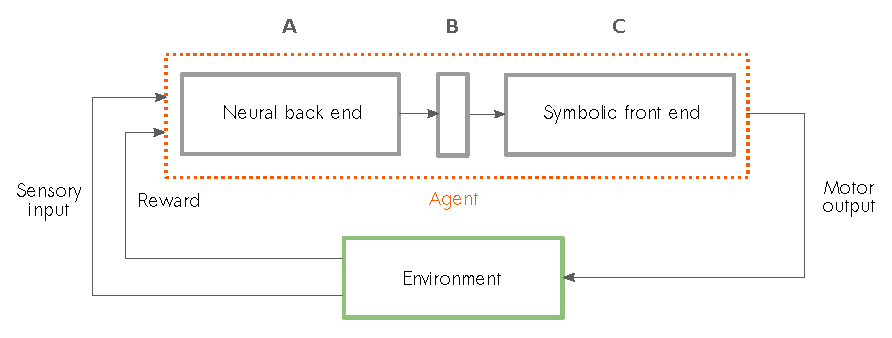
\includegraphics[width=\textwidth]{introduction/DSRL_architecture.eps}
\caption{Overview of deep symbolic reinforcement learning system architecture. \textbf{A}: The neural back end maps high-dimensional raw input data to a compositionally structured symbolic representation. \textbf{B}: The compositionally structured symbolic representation. \textbf{C}: Reinforcement learning of mapping from symbolic representation to action with maximum expected reward over time. \textit{Source: Garnelo et al.} \cite{Garnelo2016}.}
\label{fig:dsrl_archiecture}
\end{figure}

An overview of DSRL is shown in Figure \ref{fig:dsrl_archiecture}. The neural back end takes a high-dimensional input and outputs a symbolic representation. This symbolic representation is then fed to the symbolic front end, whose role is action selection. The agent then acts on the environment and obtains a reward and the sensory input of the next time step. As the neural back end learns how to represent the raw input data in a compositionally structured representation in an unsupervised manner, and the symbolic front end learns to select the action with maximum expected reward over time, the system as a whole learns end-to-end.

 TODO: Finish description of DSRL

\section{Objectives}

We'll use the image in Figure \ref{fig:dsrl_raw_input} as an example of a high-dimensional input to the neural back end. This world consists of only two shapes (circle and square) and four spaces occupied by at most one shape (top left, top right, bottom left and bottom right). The neural back end maps this raw high-dimensional input to a low-dimensional symbolic representation, shown in Table \ref{tab:dsrl_symbolic_representation}.

\begin{figure}[h!]
\centering
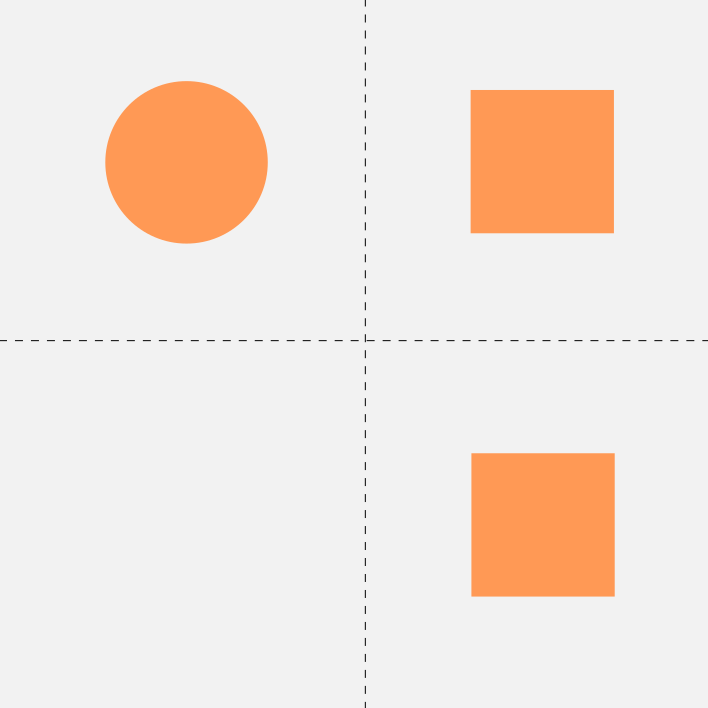
\includegraphics[scale=0.3]{introduction/DSRL_raw_input.png}
\caption{A toy example of a raw high-dimensional input.}
\label{fig:dsrl_raw_input}
\end{figure} 

% Please add the following required packages to your document preamble:
% \usepackage{booktabs}
\begin{table}[]
\centering
\label{tab:dsrl_symbolic_representation}
\begin{tabular}{@{}ll@{}}
\toprule
Type & Location   \\ \midrule
1    & {[}0, 0{]} \\
2    & {[}0, 1{]} \\
2    & {[}1, 1{]} \\ \bottomrule
\end{tabular}
\caption{Low-dimensional symbolic representation}
\end{table}

 How this is done will be explained in Chapter \ref{ch:background}, but as for now we can just take it as fact that the current method doesn't scale. That is, for very simple scenes, as in Figure ...,  This is done by passing the high-dimensional input through a series of convolutional layers and extracting the activation spectra in the latent space. These spectra are then used to classify the  

 relies on the unsupervised extraction of disentangled features, allowing for transfer learning and high-level cognitive processes. However, the unsupervised extraction of features from a wide range of scenes is still a challenge in AI research [? ]. Fortunately methods are getting better, and the first unsupervised scalable model $\beta$-VAE was developed recently.
 
 TODO: Finish objectives

\section{Contributions}

Contributions here.